\documentclass[11pt]{article}

\input{./preamble.tex}

%%
%% DOCUMENT START
%%

\begin{document}
\fancypagestyle{allpages}
{
	\fancyhf[LH]{\rightmark}
	\fancyhf[CH]{}
	\fancyhf[RH]{\thepage\hspace*{1ex}/\hspace*{1ex}\pageref{lastpage}}
	\fancyhf[LF]{}
	\fancyhf[CF]{}
	\fancyhf[RF]{}
}

\fancypagestyle{firstpage}
{
	\fancyhf[LH]{\Large Final Project \\ \large ASEN 6519: Uncertainty Quantification}
	\fancyhf[CH]{}
	\fancyhf[RH]{\large Ryan Skinner \\ \large Due 2016/??/??}
	\fancyhf[LF]{}
	\fancyhf[CF]{}
	\fancyhf[RF]{}
}

\pagestyle{allpages}
\thispagestyle{firstpage}
\renewcommand{\sectionmark}[1]{ \markright{#1}{} }

\vspace*{0in}
\begin{center}
\LARGE Impact of Geometric Uncertainty on a NACA 4412 Airfoil
\end{center}
\vspace*{0.3in}

%%%%%%%%%%%%%%%%%%%%%%%%%%%%%%%%%%%%%%%%%
%%%%%%%%%%%%%%%%%%%%%%%%%%%%%%%%%%%%%%%%%
\section{Introduction}
%%%%%%%%%%%%%%%%%%%%%%%%%%%%%%%%%%%%%%%%%
%%%%%%%%%%%%%%%%%%%%%%%%%%%%%%%%%%%%%%%%%

%%%%%%%%%%%%%%%%%%%%%%%%%%%%%%%%%%%%%%%%%
%%%%%%%%%%%%%%%%%%%%%%%%%%%%%%%%%%%%%%%%%
\section{Problem Definition}
%%%%%%%%%%%%%%%%%%%%%%%%%%%%%%%%%%%%%%%%%
%%%%%%%%%%%%%%%%%%%%%%%%%%%%%%%%%%%%%%%%%

%%%%%%%%%%%%%%%%%%%%%%%%%%%%%%%%%%%%%%%%%
%%%%%%%%%%%%%%%%%%%%%%%%%%%%%%%%%%%%%%%%%
\section{Implementation}
%%%%%%%%%%%%%%%%%%%%%%%%%%%%%%%%%%%%%%%%%
%%%%%%%%%%%%%%%%%%%%%%%%%%%%%%%%%%%%%%%%%

The shape of a 4-digit NACA xyzz airfoil is specified by three geometric parameters, all non-dimensionalized with respect to the chord length $c$:
\begin{itemize}
\item $m = \text{x} / 100$ is the maximum camber
\item $p = \text{y} / 10$ is the location of maximum camber
\item $t = \text{zz}/100$ is the maximum thickness
\end{itemize}

For a physical coordinate $x \in [0, c]$, the thickness of a symmetric airfoil is given by
\begin{equation}
y_t = 5tc\, \left[ 0.2969 \sqrt{\frac{x}{c}} + (-0.1260) \left(\frac{x}{c}\right) + (-0.3516) \left(\frac{x}{c}\right)^2 + 0.2843 \left(\frac{x}{c}\right)^3 + (-0.1015) \left( \frac{x}{c} \right)^4 \right]
\end{equation}
The coordinate pairs of points on the upper $(x_U, y_U)$ and lower $(x_L, y_L)$ surface are simply $x_U = x_L = x$, $y_U = y_t$, and $y_L = -y_t$. A symmetric airfoil corresponds to the NACA 00zz series. One example is NACA 0012, shown in \figref{fig:naca0012}.

Cambered NACA airfoils define thickness perpendicular to the camber line, which can be defined as
\begin{equation}
y_c = \begin{cases}
m \frac{x}{p^2} \left( 2p-\frac{x}{c}\right) & 0 \le x \le pc \\
m \frac{c-x}{(1-p)^2} \left(1-2p+\frac{x}{c}\right) & pc \le x \le c
\end{cases}
\end{equation}
The upper and lower coordinate pairs become
\begin{equation}
\begin{aligned}
x_U &= x - y_t \sin \theta &\quad y_U &= y_c + y_t \cos \theta \\
x_L &= x + y_t \sin \theta &\quad y_L &= y_c - y_t \cos \theta
\end{aligned}
\end{equation}
where
\begin{equation}
\theta = \arctan \left( \dd{y_c}{x} \right)
\quad \text{and} \quad
\dd{y_c}{x} =
\begin{cases}
\frac{2m}{p^2} \left( p - \frac{x}{c} \right) & 0 \le x \le pc \\
\frac{2m}{(1-p)^2} \left( p - \frac{x}{c} \right) & pc \le x \le c
\end{cases}
\end{equation}

Because cambered profiles are generated from their symmetric counterparts, we can analytically determine the displacements necessary to deform any symmetric NACA mesh into an arbitrary 4-digit NACA mesh. This results in substantial efficiency gains. In our case, we create a CAD model of a NACA 0012 airfoil, mesh it, and partition it once. Then, in the initialization stage of a new simulation, we generate a stochastic NACA realization parameterized by random variables $\mb{m}$, $\mb{p}$, and $\mb{t}$. Each mesh node on the airfoil surface is prescribed a displacement based on its $x$-coordinate, which is then passed to a linear elastic structural solver. Numerical solution of the unsteady incompressible Navier-Stokes equations proceeds on the deformed mesh.

\begin{figure}[b]
\begin{center}
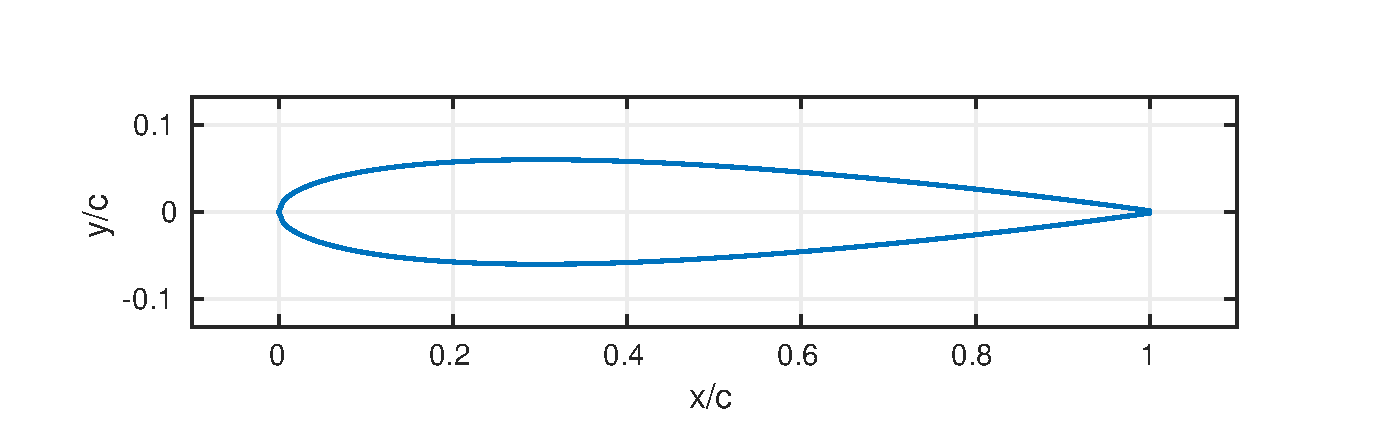
\includegraphics[width=0.85\textwidth]{naca0012.eps}
\vspace{1ex}
\caption{Surface of a NACA 0012 airfoil.}
\label{fig:naca0012}
\end{center}
\end{figure}




%%
%% DOCUMENT END
%%
\label{lastpage}
\end{document}



























